\section{Parte 0: procesos simulados}
\label{sec:parte0}

Antes de tocar datos reales conviene ver cómo se comportan la ACF y las
pruebas de ruido blanco en procesos donde la respuesta es conocida. Todo lo de
esta sección lo produce \texttt{parte0.py}, con las semillas de
\texttt{semillas.py}; las funciones $r_k$, Ljung--Box y el estimado OLS de
$\phi$ están implementadas a mano en \texttt{series.py} y son las mismas que se
usan con la serie de ventas en las Partes~3 y~4.

\subsection{Inciso 0.1: momentos del AR(1) y de la caminata aleatoria}

Sea $Y_t = c + \phi Y_{t-1} + \varepsilon_t$ con $\varepsilon_t
\overset{\text{iid}}{\sim} \mathcal{N}(0,\sigma^2)$, $|\phi|<1$, y supongamos
que el proceso es débilmente estacionario: $E[Y_t]=\mu$ y
$\operatorname{Var}(Y_t)=\gamma_0$ para todo $t$.

\paragraph{Media.} Tomando esperanza en ambos lados y usando
$E[\varepsilon_t]=0$:
\[
  \mu = E[Y_t] = c + \phi\,E[Y_{t-1}] + E[\varepsilon_t] = c + \phi\mu
  \quad\Longrightarrow\quad
  \mu(1-\phi) = c
  \quad\Longrightarrow\quad
  E[Y_t] = \frac{c}{1-\phi}.
\]
La división es válida porque $|\phi|<1$ implica $\phi\neq 1$.

\paragraph{Varianza.} $Y_{t-1}$ depende solo de
$\varepsilon_{t-1},\varepsilon_{t-2},\dots$, así que es independiente de
$\varepsilon_t$ y la covarianza entre ambos es cero. La constante $c$ no
aporta varianza. Entonces
\[
  \gamma_0 = \operatorname{Var}(c + \phi Y_{t-1} + \varepsilon_t)
  = \phi^2 \operatorname{Var}(Y_{t-1}) + \operatorname{Var}(\varepsilon_t)
  + 2\phi\operatorname{Cov}(Y_{t-1},\varepsilon_t)
  = \phi^2\gamma_0 + \sigma^2,
\]
donde se usó $\operatorname{Var}(Y_{t-1})=\operatorname{Var}(Y_t)=\gamma_0$.
Despejando,
\[
  \operatorname{Var}(Y_t) = \gamma_0 = \frac{\sigma^2}{1-\phi^2},
\]
que es positiva y finita justamente porque $\phi^2<1$.

\paragraph{Autocorrelación.} Para $k\geq 1$, $Y_{t-k}$ depende solo de choques
anteriores a $t-k+1$, así que $\operatorname{Cov}(\varepsilon_t, Y_{t-k})=0$ y
la constante no covaría con nada:
\[
  \gamma_k = \operatorname{Cov}(Y_t, Y_{t-k})
  = \operatorname{Cov}(c + \phi Y_{t-1} + \varepsilon_t,\; Y_{t-k})
  = \phi\,\operatorname{Cov}(Y_{t-1}, Y_{t-k})
  = \phi\,\gamma_{k-1}.
\]
El último paso usa la estacionariedad: la covarianza entre $Y_{t-1}$ y
$Y_{t-k}$ solo depende de su separación, $k-1$. Iterando la recursión desde
$\gamma_0$ se obtiene $\gamma_k = \phi^k\gamma_0$, y por lo tanto
\[
  \rho_k = \frac{\gamma_k}{\gamma_0} = \phi^k .
\]

\paragraph{Caminata aleatoria.} Con $\phi=1$, $c=0$ y $Y_0=0$, sustituyendo
hacia atrás,
\[
  Y_t = Y_{t-1} + \varepsilon_t = Y_{t-2} + \varepsilon_{t-1} + \varepsilon_t
  = \dots = Y_0 + \sum_{i=1}^{t}\varepsilon_i = \sum_{i=1}^{t}\varepsilon_i .
\]
Los $\varepsilon_i$ son independientes, así que la varianza de la suma es la
suma de las varianzas:
\[
  \operatorname{Var}(Y_t) = \sum_{i=1}^{t}\operatorname{Var}(\varepsilon_i)
  = t\sigma^2 .
\]
La media sí es constante ($E[Y_t]=0$), pero la varianza crece linealmente con
$t$: depende del momento en que se observa, y eso viola directamente la
condición $\operatorname{Var}(Y_t)=\sigma^2$ para todo $t$ de la
estacionariedad débil. Dicho de otra forma, la fórmula
$\sigma^2/(1-\phi^2)$ explota cuando $\phi\to 1$: no existe una varianza
estacionaria a la cual converger. Tampoco la autocorrelación es función solo
del rezago: $\operatorname{Corr}(Y_t,Y_{t-k}) = \sqrt{(t-k)/t}$, que depende
de $t$.

\subsection{Inciso 0.2: simulación del AR(1)}

La función \texttt{simular\_ar1} genera $200+300$ pasos de un AR(1) con $c=0$
y $\sigma=1$ a partir de $Y_0=0$ y descarta los primeros 200. Con $|\phi|<1$
el efecto del valor inicial decae como $\phi^t$; a los 200 pasos, incluso con
$\phi=0.9$, queda $0.9^{200}\approx 7\times10^{-10}$ del valor inicial, así
que la serie que se conserva ya está en su distribución estacionaria. Con
$\phi=1$ eso no funciona: la serie conservada es $Y_t = Y_{200} +
\sum_{i=201}^{t}\varepsilon_i$, una caminata aleatoria que arranca en
$Y_{200}$ en lugar de 0, y la varianza sigue creciendo sin límite. Pero el
punto de arranque no afecta a $r_k$: sumar una constante a toda la serie mueve
también a $\bar y$ y deja intactas las desviaciones $y_t-\bar y$, que son lo
único que entra en la fórmula. Por eso descartar o no los 200 pasos no cambia
en nada los resultados de $r_k$ para la caminata.

La figura~\ref{fig:p0_realizaciones} muestra una realización de cada
proceso. Con $\phi=0$ la serie no tiene ninguna inercia; con $\phi=0.5$
aparecen rachas cortas; con $\phi=0.9$ la serie pasa decenas de pasos de un
mismo lado de cero, aunque siempre regresa; y con $\phi=1$ nunca regresa: se
aleja de su origen (nótese que arranca en $Y_{200}\neq0$) y lo que en un AR
estacionario serían fluctuaciones aquí parece una tendencia.

\begin{figure}[H]
  \centering
  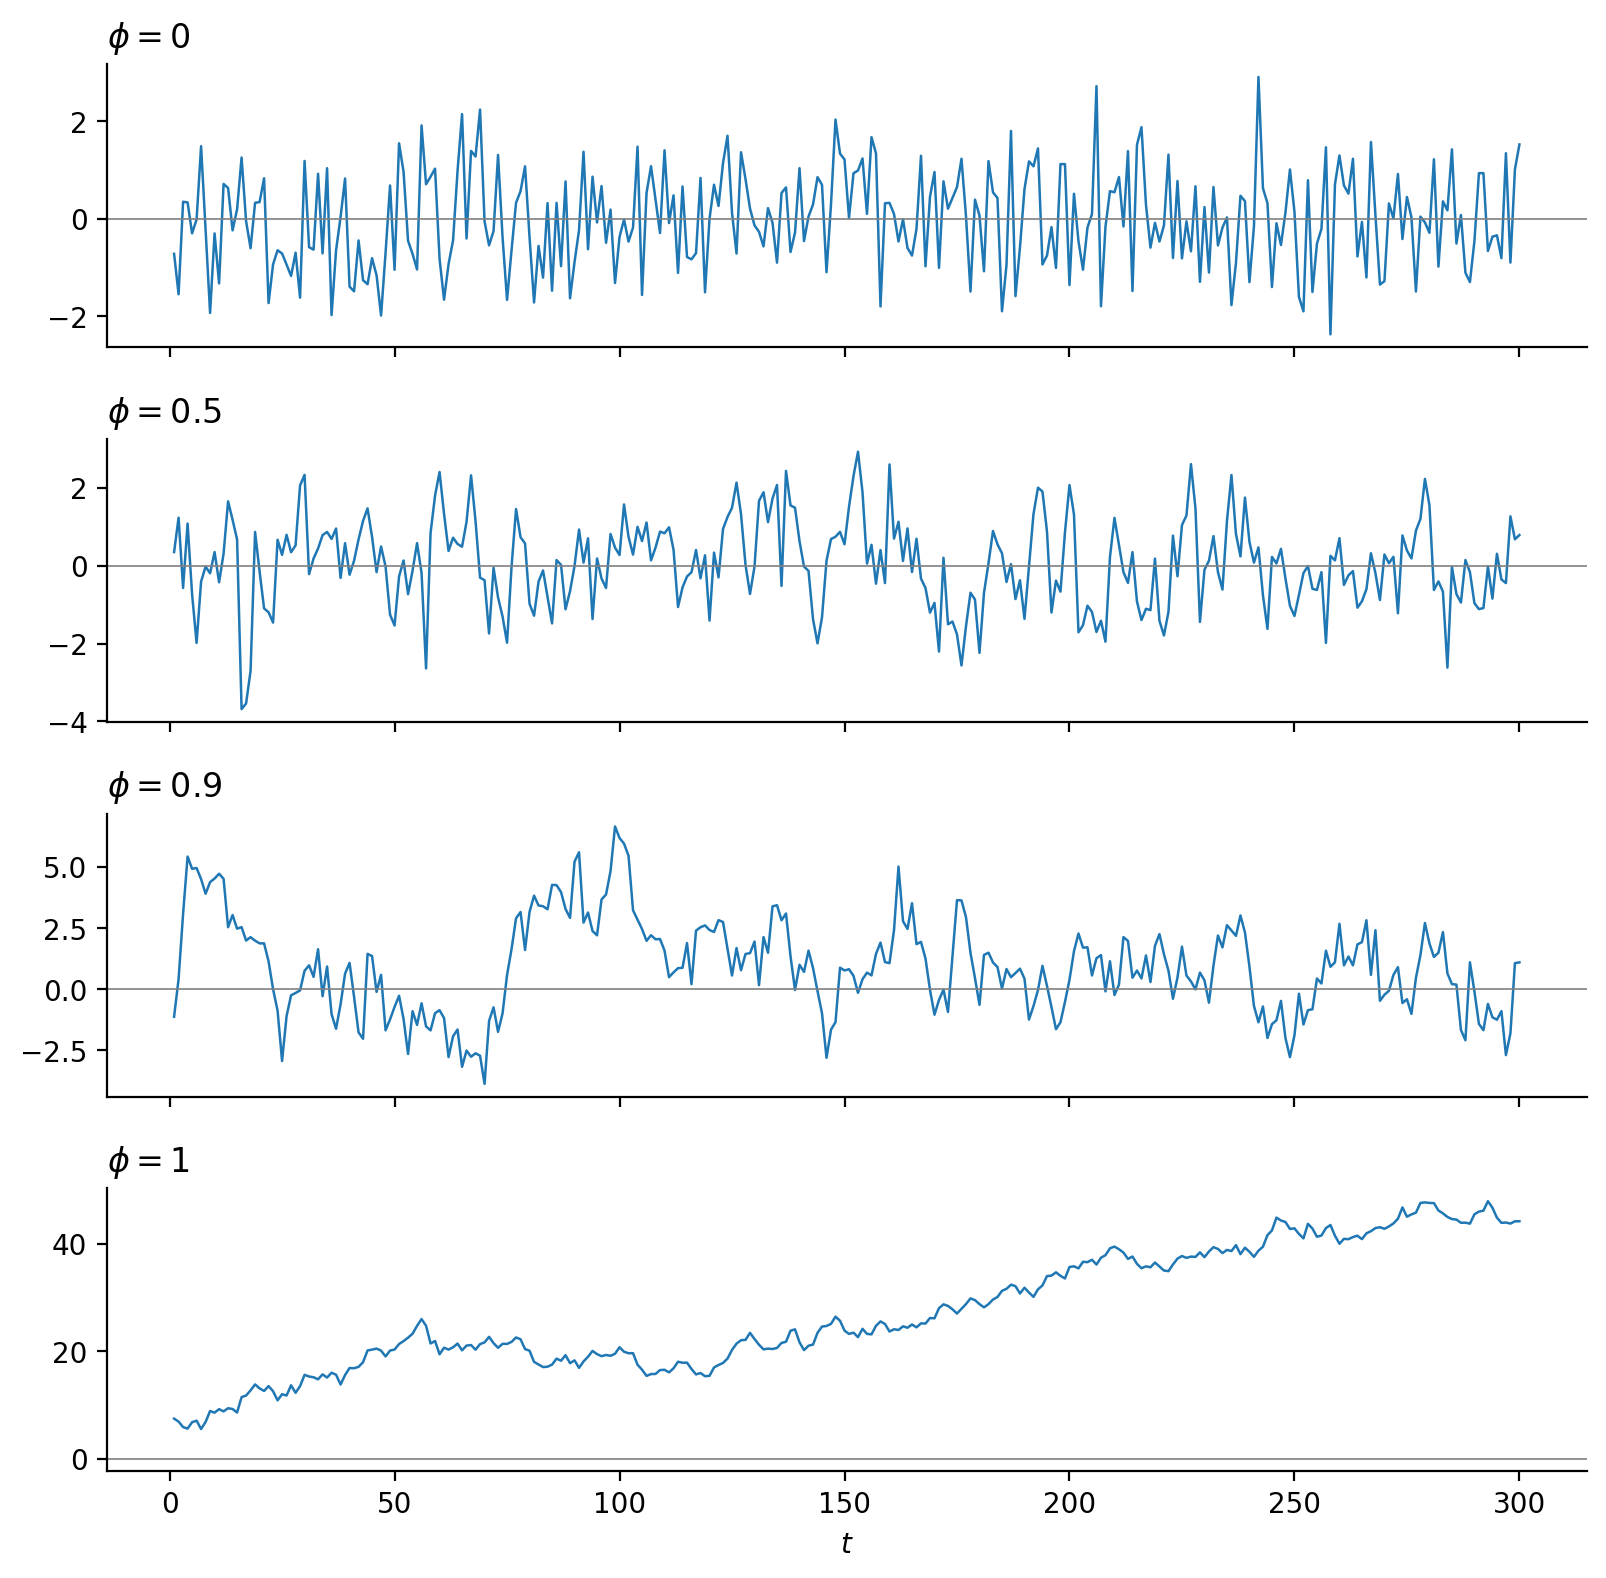
\includegraphics[width=0.85\textwidth]{p0_realizaciones_ar1.png}
  \caption{Una realización de 300 pasos de cada AR(1), después de descartar
  200 pasos de arranque. La escala vertical cambia entre paneles: la varianza
  estacionaria $1/(1-\phi^2)$ vale 1, 1.33 y 5.26 para $\phi=0,0.5,0.9$, y no
  existe para $\phi=1$.}
  \label{fig:p0_realizaciones}
\end{figure}

La tabla~\ref{tab:p0_ar1} resume las 5\,000 réplicas por escenario. Cada
celda es el promedio sobre réplicas y, entre paréntesis, su error estándar
$s/\sqrt{5000}$. La tasa de rechazo es la fracción de réplicas en que
$|r_1|>1.96/\sqrt{300}=0.113$, es decir, en que la prueba de retardo 1 de la
Tarea~2 declara que la serie no es ruido blanco.

\begin{table}[H]
  \centering
  \small
  \begin{tabular}{cccccc}
\toprule
$\phi$ & $\bar r_1$ & $\bar r_5$ & $\phi^5$ & Rechazo $|r_1|>1.96/\sqrt{n}$ & $\bar{\hat\phi}_{\text{OLS}}$ \\
\midrule
0 & -0.002 (0.001) & -0.003 (0.001) & 0.000 & 0.046 (0.003) & -0.002 (0.001) \\
0.5 & 0.491 (0.001) & 0.020 (0.001) & 0.031 & 1.000 (0.000) & 0.492 (0.001) \\
0.9 & 0.884 (0.000) & 0.534 (0.001) & 0.590 & 1.000 (0.000) & 0.887 (0.000) \\
1 & 0.976 (0.000) & 0.883 (0.001) & 1.000 & 1.000 (0.000) & 0.982 (0.000) \\
\bottomrule
\end{tabular}

  \caption{AR(1) con $n=300$ y 5\,000 réplicas por valor de $\phi$. Promedio
  (error estándar).}
  \label{tab:p0_ar1}
\end{table}

\subsection{Inciso 0.3: lo que dice la tabla}

\paragraph{Ruido blanco.} Con $\phi=0$ la prueba rechaza en el 4.62\% de las
réplicas, con error estándar de 0.30 puntos: está a poco más de un error
estándar del 5\% nominal, que es lo esperado. La prueba está construida
precisamente para equivocarse un 5\% de las veces cuando la hipótesis nula es
cierta, y aquí la nula es cierta por construcción. Que quede un poco por debajo
de 5\% tiene además una razón teórica: bajo ruido blanco, $E[r_1]\approx-1/n$
y $\operatorname{Var}(r_1)\approx (n-1)/(n(n+2))$, ligeramente menor que la
$1/n$ con que se dibujan las bandas, así que la tasa exacta ronda 4.9\%. El
$\bar r_1=-0.0023$ observado también es compatible con $-1/300=-0.0033$.

\paragraph{Caminata aleatoria.} La teoría estacionaria diría $\rho_5=\phi^5=1$,
pero el promedio de $r_5$ es 0.883. No es un error de simulación (el error
estándar es 0.001): para una caminata aleatoria la ACF muestral está
fuertemente sesgada hacia abajo. La razón es que $r_k$ mide desviaciones
respecto a $\bar y$, y en una caminata $\bar y$ es una media que no
representa a ningún tramo de la serie: la serie se pasa largos periodos de un
lado y luego del otro. Además el denominador usa los $n$ términos y el
numerador solo $n-k$. De hecho, la fórmula $\rho_k=\phi^k$ ni siquiera
aplica, porque la derivación del inciso 0.1 supuso estacionariedad. Lo que sí
se ve es la huella visual que menciona el enunciado: la ACF de la caminata
baja muy despacio ($\bar r_1=0.976$, $\bar r_5=0.883$), mientras que con
$\phi=0.5$ el valor ya cayó a casi cero en el rezago 5. Para los procesos
estacionarios el sesgo de $r_5$ también existe pero es menor: con $\phi=0.9$
se obtiene 0.534 contra $0.9^5=0.590$, y con $\phi=0.5$, 0.020 contra 0.031.

\paragraph{Sesgo del estimado OLS.} El estimado OLS de $\phi$ queda
sistemáticamente por debajo del valor verdadero, y el sesgo crece con $\phi$:
$-0.002$ para $\phi=0$, $-0.008$ para $0.5$, $-0.013$ para $0.9$ y $-0.018$
para $1$, todos varias veces mayores que su error estándar. Es el sesgo de
Hurwicz: en una autorregresión el regresor $y_{t-1}$ no es independiente de
los errores pasados, y la aproximación clásica $E[\hat\phi]-\phi\approx
-(1+3\phi)/n$ da $-0.003$, $-0.008$ y $-0.012$ para los tres casos
estacionarios, muy cerca de lo observado. El estimador es consistente: el
sesgo es de orden $1/n$ y desaparece cuando la muestra crece, aunque con 300
observaciones todavía se nota. En la caminata, la teoría de Dickey--Fuller
dice que $\hat\phi$ converge todavía más rápido (a ritmo $1/n$ en vez de
$1/\sqrt n$) pero con una distribución asimétrica, cargada hacia valores
menores que 1, y eso es lo que se ve en el $0.982$.

\subsection{Inciso 0.4: las dos razones para reprobar}

Ahora $Y_t=m_t+\varepsilon_t$ no tiene ninguna memoria: los $\varepsilon_t$
son independientes y $m_t$ es determinista. La
figura~\ref{fig:p0_sin_memoria} muestra una realización de cada proceso y la
tabla~\ref{tab:p0_sin_memoria} repite la tabla del inciso 0.2 agregando
$\bar r_7$; la primera fila es el ruido blanco del inciso anterior, como
referencia.

\begin{figure}[H]
  \centering
  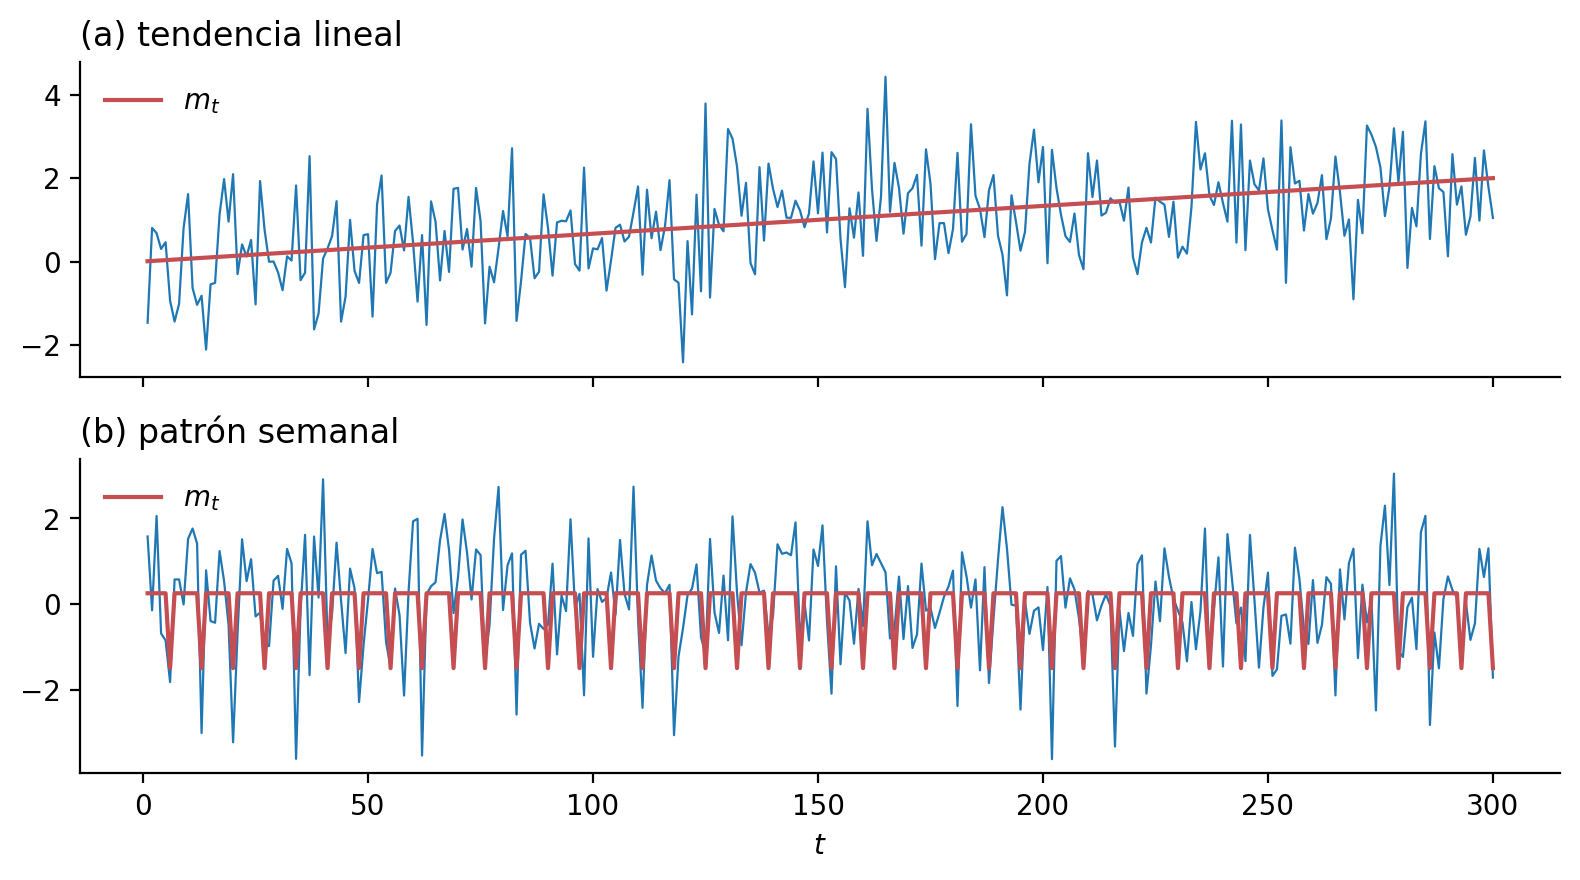
\includegraphics[width=0.85\textwidth]{p0_realizaciones_sin_memoria.png}
  \caption{Procesos sin memoria con media variable. En rojo, la media $m_t$.}
  \label{fig:p0_sin_memoria}
\end{figure}

\begin{table}[H]
  \centering
  \small
  \begin{tabular}{lccccc}
\toprule
Proceso & $\bar r_1$ & $\bar r_5$ & $\bar r_7$ & Rechazo $r_1$ & $\bar{\hat\phi}_{\text{OLS}}$ \\
\midrule
Ruido blanco ($\phi=0$) & -0.002 (0.001) & -0.003 (0.001) & -0.004 (0.001) & 0.046 (0.003) & -0.002 (0.001) \\
(a) Tendencia & 0.246 (0.001) & 0.235 (0.001) & 0.230 (0.001) & 0.986 (0.002) & 0.247 (0.001) \\
(b) Semanal & -0.047 (0.001) & -0.050 (0.001) & 0.266 (0.001) & 0.112 (0.004) & -0.048 (0.001) \\
\bottomrule
\end{tabular}

  \caption{Procesos sin memoria, $n=300$, 5\,000 réplicas. Promedio (error
  estándar).}
  \label{tab:p0_sin_memoria}
\end{table}

\paragraph{La tendencia reprueba sin tener memoria.} La serie con tendencia
rechaza la prueba de retardo 1 en el 98.6\% de las réplicas, y el OLS le
asigna $\hat\phi\approx0.25$ a un proceso cuyo $\phi$ verdadero es cero. Se
puede predecir el número: $m_t$ recorre $[0,2]$ de forma casi uniforme, con
varianza $\approx 4/12=1/3$, y como dos días cercanos tienen casi la misma
$m_t$, la covarianza entre vecinos es esa misma varianza; así $r_k\approx
(1/3)/(1/3+1)=0.25$ para todo rezago pequeño. Eso es exactamente lo que dice
la tabla: $\bar r_1=0.246$, $\bar r_5=0.235$, $\bar r_7=0.230$, una ACF que
casi no decae. Es la razón (2) del enunciado: $\bar y$ no es la media de nadie,
los días del final quedan todos por encima y los del inicio todos por debajo, y
eso se ve como correlación.

\paragraph{El patrón semanal pasa aunque tenga estructura.} La serie semanal
rechaza solo en el 11.2\% de las réplicas, poco más que el ruido blanco, y su
$\bar r_1=-0.047$ es diminuto. De nuevo se puede calcular: sobre un ciclo de 7
días $m_t$ tiene media 0 y varianza $(6\cdot0.25^2+1.5^2)/7=0.375$, pero
la covarianza entre días consecutivos es solo
$(5\cdot0.25^2-2\cdot0.375)/7=-0.0625$, y $r_1\approx-0.0625/1.375=-0.045$.
Toda la estructura está a distancia 7: un domingo se parece al domingo
anterior, no al sábado. Por eso $\bar r_7=0.266$ (la predicción es
$0.375/1.375=0.273$), mientras que $r_1$ y $r_5$ están cerca de cero.

\paragraph{Conexión con RANDU.} Es el mismo fenómeno que con RANDU en la
Tarea~2: RANDU pasaba las pruebas unidimensionales y de pares consecutivos y,
sin embargo, sus ternas caían en solo 15 planos, porque su dependencia vivía en
una combinación de los rezagos 1 y 2 que esas pruebas no miran. La prueba de
retardo 1 solo puede ver estructura en el rezago 1; un proceso con la
dependencia en otro lado (el rezago 7, o una combinación lineal de rezagos)
la pasa sin problema. Pasar una prueba nunca demuestra independencia: solo
dice que en la dirección que esa prueba mira no se encontró nada.

\subsection{Inciso 0.5: la prueba que sí ve}

La tabla~\ref{tab:p0_ljungbox} compara la tasa de rechazo de la prueba de
retardo 1 con la de Ljung--Box al 5\%, con $m=10$ (la recomendación de FPP2
sin estacionalidad) y con $m=6\approx\log(300)=5.7$ (la sugerencia de Tsay).
La implementación propia coincide con
\nolinkurl{statsmodels.stats.diagnostic.acorr_ljungbox} hasta el sexto decimal
en el estadístico y en el valor-$p$; \texttt{parte0.py} lo verifica con un
\texttt{assert} en una réplica de cada proceso.

\begin{table}[H]
  \centering
  \small
  \begin{tabular}{lccc}
\toprule
Proceso & Rechazo $r_1$ & LB $m=10$ & LB $m=6$ \\
\midrule
Ruido blanco ($\phi=0$) & 0.046 (0.003) & 0.053 (0.003) & 0.053 (0.003) \\
(a) Tendencia & 0.986 (0.002) & 1.000 (0.000) & 1.000 (0.000) \\
(b) Semanal & 0.112 (0.004) & 0.956 (0.003) & 0.209 (0.006) \\
\bottomrule
\end{tabular}

  \caption{Tasa de rechazo al 5\% sobre 5\,000 réplicas, $n=300$. Promedio
  (error estándar).}
  \label{tab:p0_ljungbox}
\end{table}

Con ruido blanco las dos versiones de Ljung--Box rechazan alrededor del 5\%
(5.3\%), como deben. Con la tendencia rechazan siempre, igual que la prueba de
retardo 1: ahí la estructura se ve en todos los rezagos.

El cambio está en el patrón semanal. Ljung--Box con $m=10$ lo rechaza en el
95.6\% de las réplicas, contra el 11.2\% de la prueba de retardo 1, porque
$Q(10)$ suma $r_k^2$ para $k=1,\dots,10$ y eso incluye el $r_7\approx0.27$
que la prueba de retardo 1 no mira; elevado al cuadrado y multiplicado por
$n(n+2)/(n-7)$, ese solo término aporta alrededor de 22 al estadístico, cuando
el valor crítico de una $\chi^2_{10}$ al 5\% es 18.3. En cambio, con $m=6$ la
tasa cae a 20.9\%: seis rezagos no llegan al 7, así que $Q(6)$ es casi tan
ciego como la prueba de retardo 1. Esta es la comparación que pedía el
enunciado entre las dos reglas para escoger $m$, y la lección es que $m$ tiene
que cubrir al menos el periodo estacional; por eso FPP2 recomienda $m=2s$
cuando hay estacionalidad. Con datos diarios de una tienda, la regla
$m\approx\log n$ por sí sola no es suficiente.
